\documentclass{article}
\usepackage{amsmath}
\usepackage{amssymb}
\usepackage[a4paper, top=25mm, bottom=25mm, left=25mm, right=25mm]{geometry}
\usepackage{pgfplots}
\pgfplotsset{compat=1.18}
\usepackage{mathtools}
\usepgfplotslibrary{polar}
\usepgfplotslibrary{fillbetween}

\begin{document}
\pagestyle{empty}
\large

\begin{center}
2024-2025 Spring \\MAT124 Final\\(18/06/2025)
\end{center}

\noindent 1. Let $f(x,y)=6-x^2-y^2$. Find the tangent plane and normal line equations (symmetric or parametric equations) of the graph of $f$ at the point $P(1,2,1)$.

\hfill

\noindent 2. Find all critical points of the given function $f(x,y)=x^3+y^3-3xy+2$ and classify them (i.e., determine whether each critical point corresponds to a local maximum, local minimum, or saddle point).

\hfill

\noindent 3. Find the maximum and minimum of the function $f(x,y)=81x^2+y^2$ subject to the given constraint $4x^2+y^2=9$ using Lagrange multipliers.

\hfill

\noindent 4. The equation $z^3-zy^2+yx=3$ defines $z$ implicitly as a function of $x$ and $y$. It is given that $z=2$ when $(x,y)=(-3,1)$. Evaluate $\displaystyle\frac{\partial z}{\partial x}$ and $\displaystyle\frac{\partial z}{\partial y}$ at $(-3,1)$.

\hfill

\noindent 5.

\hfill

\noindent (a) Reverse the order of integration and evaluate the double integral.

\[\int_0^{\sqrt2}\int_0^{2-x^2}x\mathrm{e}^{x^2}\,dy\,dx\]
 
\hfill

\noindent (b) Evaluate the double integral

\[\iint_R \frac{2xy}{x^2+y^2}\,dA\]

\hfill

\noindent where the region $R = \{(x,y): x\geq0,\:y\geq0,\:z\geq0,\:x^2+y^2\leq a^2\}$

\hfill

\noindent 6. 

\hfill

\noindent (a) Convert the triple integral into cylindrical coordinates. Do not evaluate the integral.

\[\int_{-1}^1\int_0^{\sqrt{1-y^2}}\int_{x^2+y^2}^{\sqrt{x^2+y^2}}xyz\,dz\,dx\,dy\]

\hfill

\noindent (b) Use a triple integral in spherical coordinates in order to find the volume of the sphere centered at $(0,0,0)$ with radius $3$.

\hfill

\noindent 7.

\hfill

\noindent (a) Determine whether the vector field $\mathbf{F}(x,y,z)=y\,\mathbf{i}+x\,\mathbf{j}+z^2\,\mathbf{k}$ is conservative and find a potential if it is conservative.

\hfill

\noindent (b) Evaluate the line integral $\int_C\mathbf{F}\cdot d\mathbf{r}$ for the vector field $\mathbf{F}(x,y,z)=z\,\mathbf{i}-y\,\mathbf{j}+2x\,\mathbf{k}$ along the curve $x=t,\:y=t^2\:z=t^3$ from $(0,0,0)$ to $(1,1,1)$.

\newpage

\begin{center}
2024-2025 Spring Final (18/06/2025) Solutions\\
(Last update: 08/08/2025 00:21)
\end{center}

\noindent 1. The equation of the tangent plane at a point on the surface and the normal line to this plane are given, respectively, by

\begin{equation}z-z_0=f_x(x_0,y_0)(x-x_0)+f_y(x_0,y_0)(y-y_0)\end{equation}

\begin{equation}
\left.\begin{array}{c}
x=x_0+f_x(x_0,y_0)\cdot t\\
y=y_0+f_y(x_0,y_0)\cdot t\\
z=z_0- t\\
\end{array}\right\}\quad-\infty<t<\infty
\end{equation}

\hfill

\noindent Calculate the first partial derivatives of $f$.

\[f_x=-2x,\quad f_y=-2y\quad\implies\quad f_x(1,2)=-2,\quad f_y(1,2)=-4\]

\hfill

\noindent Using $(1)$ and $(2)$ determine the equations.

\[\boxed{\begin{array}{l}
\text{Tangent plane equation: } z-1=-2(x-1)-4(y-2)\implies z=-2x-4y+11\\[1em]
\text{Normal line equation:}\:\left.\begin{array}{l}
x=1-2t\\
y=2-4t\\
z=1-t\\
\end{array}\right\}\quad-\infty<t<\infty
\end{array}
}
\]

\hfill

\noindent 2. To identify the critical points, find where both $f_x=f_y=0$ or one of the partial derivatives does not exist.

\[f_x=3x^2-3y,\quad f_y=3y^2-3x\]
\[\left.\begin{array}{c}
f_x=0\implies 3y=3x^2\implies y=x^2\\
f_y=0\implies 3y^2=3x\implies x=y^2 
\end{array}\:\right\}\: x=x^4\implies x(x^3-1)=0\implies x_1=0,\quad x_2=1\]

\[x_1=0\implies y_1=0,\quad x_2=1\implies y_2=1\]

\hfill

\noindent The critical points are $(0,0)$ and $(1,1)$. To classify these points, calculate the second partial derivatives and then find the Hessian determinants.

\[f_{xx}=6x,\quad f_{xy}=f_{yx}=-3,\quad f_{yy}=6y\]

\[(0,0)\rightarrow\left\{\:\begin{array}{l}
f_{xx}=0,\quad f_{xy}=-3,\quad f_{yy}=0\\[1em]
\left|\begin{array}{cc}
0 & -3\\
-3 & 0
\end{array}\right|=0\cdot0-(-3)\cdot(-3)=-9<0
\end{array}\right.\]

\[(1,1)\rightarrow\left\{\:\begin{array}{l}
f_{xx}=6,\quad f_{xy}=-3,\quad f_{yy}=6\\[1em]
\left|\begin{array}{cc}
6 & -3\\
-3 & 6
\end{array}\right|=6\cdot6-(-3)\cdot (-3)=27>0,\quad f_{xx}>0
\end{array}\right.\]

\[\boxed{\text{A local minimum occurs at }(1,1)\text{ and a saddle point occurs at }(0,0).}\]

\newpage

\noindent 3. Let $g(x,y)=4x^2+y^2-9$ be the constraint. Solve the system of equations below.

\[
\left.
\begin{array}{c}
\displaystyle\nabla f=\lambda\nabla g\\
\displaystyle g(x,y)=0
\end{array}
\right\}\quad
\begin{array}{l}
\nabla f=\left\langle162x,2y\right\rangle=\lambda\left\langle8x,2y\right\rangle=\lambda\nabla g
\end{array}
\]

\hfill

\[2y=2\lambda y\implies 2y(1-\lambda)=0\implies y=0\quad\text{or}\quad\lambda=1\]
\[162x=8\lambda x\implies 2x(81-4\lambda)=0\implies x=0\quad\text{or}\quad\lambda=\frac{81}4\]

\[y=0\implies g(x,0)=4x^2+0^2-9=0\implies x=\pm\frac32\]
\[x=0\implies g(0,y)=4\cdot0^2+y^2=9\implies y=\pm3\]

\hfill

\noindent Evaluate $f$ at the points $\displaystyle(0,3),\:(0,-3),\:\left(\frac32,0\right),\:\left(-\frac32,0\right)$ and compare them all.

\[f\left(0,3\right)=81\cdot0^2+3^2=9,\quad f\left(0,-3\right)=81\cdot0^2+(-3)^2=9\]

\[f\left(\frac32,0\right)=81\cdot\left(\frac32\right)^2+0^2=\frac{729}4,\quad f\left(-\frac32,0\right)=81\cdot\left(-\frac32\right)^2+0^2=\frac{729}4\]

\[\boxed{\text{The minimum value is }9,\text{ the maximum value is }\frac{729}4.}\]

\hfill

\noindent 4. Obtain the partial derivatives of both sides.

\[3z^2\cdot z_x-z_x\cdot y^2+y=0\implies z_x=\frac{-y}{3z^2-y^2}\bigg|_{(-3,1,2)}=-\frac1{11}\]

\[3z^2\cdot z_y-z_y\cdot y^2-2zy+x=0\implies z_y=\frac{2zy-x}{3z^2-y^2}\bigg|_{(-3,1,2)}=\frac7{11}\]

\[\boxed{\frac{\partial z}{\partial x}=-\frac1{11},\quad\frac{\partial z}{\partial y}=\frac7{11}}\]

\hfill

\noindent 5.

\hfill

\noindent (a)
\begin{center}
\begin{minipage}{0.4\textwidth}
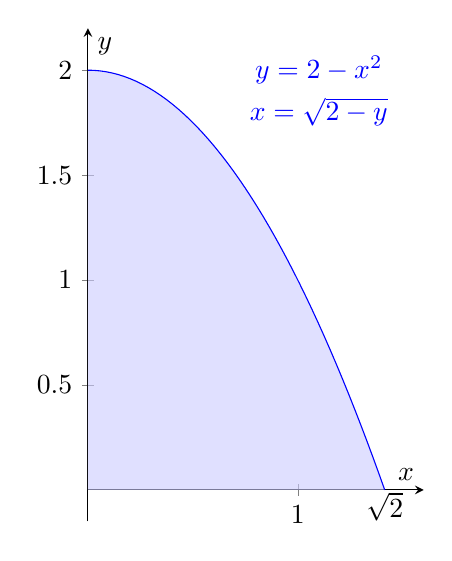
\begin{tikzpicture}
  \begin{axis}[
    axis equal image,
    xlabel=$x$, ylabel=$y$,
    xmin=0, xmax=1.6,
    ymin=-0.15, ymax=2.2,
    xtick={-2,-1,1,2},
    domain=2:2,
    samples=50,
    axis lines=middle,
    clip=true,
    scale=1.1,
    ]
    \addplot[domain=0:1.4143, blue] {2-x^2};
    
    \addplot[domain=0:1.4143, draw=none, name path=A] {0};
    \addplot[domain=0:1.4143, draw=none, name path=B] {2-x^2};
    \addplot[domain=0:1.4143, opacity=0.6, blue!20] fill between[of=A and B];

    \node[blue] at (1.1,2) {$y=2-x^2$};
    \node[blue] at (1.1,1.8) {$x=\sqrt{2-y}$};
    \node at (1.4143,-0.08) {$\sqrt2$};
  \end{axis}
\end{tikzpicture}
\end{minipage}\begin{minipage}{0.58\textwidth}
\begin{align*}\mathrm{I}&=\int_0^{\sqrt2}\int_0^{2-x^2}x\mathrm{e}^{x^2}\,dy\,dx=\int_0^2\int_0^{\sqrt{2-y}}x\mathrm{e}^{x^2}\,dx\,dy\\\\&=\int_0^2\left[\frac{\mathrm{e}^{x^2}}2\right]_{x=0}^{x=\sqrt{2-y}}\,dy=\frac12\int_0^2\left(\mathrm{e}^{2-y}-1\right)\,dy\\\\&=\frac12\left[-\mathrm{e}^{2-y}-y\right]_0^2=\boxed{\frac{\mathrm{e}^2-3}2}\end{align*}
\end{minipage}
\end{center}

\hfill

\noindent (b)
\begin{center}
\begin{minipage}{0.35\textwidth}
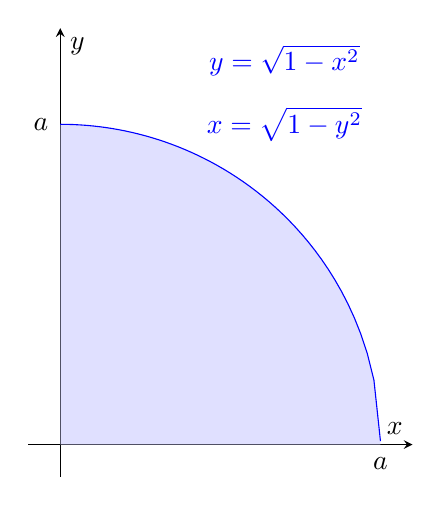
\begin{tikzpicture}
  \begin{axis}[
    axis equal image,
    xlabel=$x$, ylabel=$y$,
    xmin=-0.1, xmax=1.1,
    ymin=-0.1, ymax=1.3,
    xtick=\empty, ytick=\empty,
    domain=2:2,
    samples=50,
    axis lines=middle,
    clip=true,
    scale=1,
    ]
    \addplot[domain=0:1, blue] {sqrt(1-x^2)};
    
    \addplot[domain=0:1, draw=none, name path=A] {0};
    \addplot[domain=0:1, draw=none, name path=B] {sqrt(1-x^2)};
    \addplot[domain=0:1, opacity=0.6, blue!20] fill between[of=A and B];

    \node[blue] at (0.7,1.2) {$y=\sqrt{1-x^2}$};
    \node[blue] at (0.7,1) {$x=\sqrt{1-y^2}$};
    \node at (1,-0.06) {$a$};
    \node at (-0.06,1) {$a$};
  \end{axis}
\end{tikzpicture}
\end{minipage}\begin{minipage}{0.5\textwidth}
\[\iint_R\frac{2xy}{x^2+y^2}\,dA=\int_0^a\int_0^{\sqrt{1-x^2}}\frac{2xy}{x^2+y^2}\,dy\,dx\]
\end{minipage}
\end{center}

\hfill

\noindent Notice that it would be difficult to solve the integral in rectangular coordinates. We may switch to polar coordinates to easily evaluate the integral.

\[x=r\cos\theta,\quad y=r\sin\theta,\quad x^2+y^2=r^2,\quad dA=r\,dr\,d\theta\]

\begin{align*}\mathrm{I}&=\iint_R\frac{2xy}{x^2+y^2}\,dA=\int_0^{\textstyle\frac\pi2}\int_0^a\frac{2r\cos\theta\cdot r\sin\theta}{\left(r\cos\theta\right)^2+\left(r\sin\theta\right)^2}\,r\,dr\,d\theta\\\\&=\int_0^{\textstyle\frac\pi2}\int_0^a\frac{2r^3\cos\theta\sin\theta}{r^2(\sin^2\theta+\cos^2\theta)}\,dr\,d\theta=\int_0^{\textstyle\frac\pi2}\int_0^a r \sin(2\theta)\,dr\,d\theta=\int_0^{\textstyle\frac\pi2}\sin(2\theta)\left[\frac{r^2}2\right]_{r=0}^{r=a}\,d\theta\\\\&=\frac{a^2}2\int_0^{\textstyle\frac\pi2}\sin(2\theta)\,d\theta=\frac{a^2}2\left[\frac{-\cos(2\theta)}2\right]_0^{\textstyle\frac\pi2}=\frac{a^2}4\left(-\cos\pi+\cos0\right)=\boxed{\frac{a^2}2}\end{align*}

\noindent 6.

\hfill

\noindent (a) Use the transformation below.
\[
\begin{array}{c}
z=z\\
x=r\cos\theta\\
y=r\sin\theta\\
r^2=x^2+y^2\\
dV=r\,dz\,dr\,d\theta
\end{array}\quad\rightarrow\quad
\begin{array}{c}
\sqrt{x^2+y^2}=\sqrt{r^2}=r=z_{\text{upper}}\\
x^2+y^2=r^2=z_{\text{lower}}\\
\displaystyle-1<y<1,\:<x<\sqrt{1-y^2}\implies0\leq r\leq1,\:-\frac\pi2\leq\theta\leq\frac\pi2\\
xyz=r\cos\theta\cdot r\sin\theta\cdot z
\end{array}
\]

\[\boxed{\int_{-\pi/2}^{\pi/2}\int_0^1\int_{r^2}^rzr^3\sin\theta\cos\theta\,dz\,dr\,d\theta}\]

\hfill

\noindent (b) We have the sphere $x^2+y^2+z^2=9$. Use the transformation below.

\[
\begin{array}{c}
z=\rho\cos\phi\\
r=\rho\sin\phi\\
x^2+y^2+z^2=\rho^2\\
dV=\rho^2\sin\phi\,d\rho\,d\phi\,d\theta
\end{array}\quad\rightarrow\quad
\begin{array}{c}
x^2+y^2+z^2=9\implies\rho^2=9\implies\rho=3\\[1em]
0\leq\theta\leq2\pi,\quad0\leq\phi\leq2\pi
\end{array}
\]

\begin{align*}
\text{Volume}&=\int_0^{2\pi}\int_0^{2\pi}\int_0^{3}\rho^2\sin\phi\,d\rho\,d\phi\,d\theta=\int_0^{2\pi}\int_0^{2\pi}\sin\phi\cdot\left[\frac{\rho^3}3\right]_{\rho=0}^{\rho=3}\,d\phi\,d\theta\\\\&=\int_0^{2\pi}\int_0^{2\pi}9\sin\phi\,d\phi\,d\theta=\int_0^{2\pi}\bigg[-9\cos\phi\bigg]_{\phi=0}^{\phi=2\pi}\,d\theta\\\\&=\int_0^{2\pi}\left(-9\cos(2\pi)+9\cos0\right)\,d\theta=\int_0^{2\pi}18\,d\theta=18\bigg[\theta\bigg]_0^{2\pi}=\boxed{36\pi}
\end{align*}

\noindent 7.

\hfill

\noindent (a) Assume that $\nabla f=\mathbf{F}$ for some potential function $f$. Then, the mixed partial derivatives of the components must be equal.

\[
\begin{array}{c}
\displaystyle\frac{\partial\mathrm{F}_1}{\partial y}=1=\frac{\partial\mathrm{F}_2}{\partial x},\quad\frac{\partial\mathrm{F}_1}{\partial z}=0=\frac{\partial\mathrm{F}_3}{\partial x},\quad\frac{\partial\mathrm{F}_2}{\partial z}=0=\frac{\partial\mathrm{F}_3}{\partial y}
\end{array}
\]

\hfill

\noindent This means $\mathbf{F}$ is conservative on its domain.

\[\frac{\partial f}{\partial x}=y,\quad\frac{\partial f}{\partial y}=x,\quad\frac{\partial f}{\partial z}=z^2\]

\[\int\frac{\partial f}{\partial x}\,dx=\int y\,dx=xy+g(y,z)=f(x,y,z)\]

\begin{align*}\frac{\partial f}{\partial y}&=\frac{\partial}{\partial y}\left(xy+g(y,z)\right)=x+g_y(y,z)=x\implies g_y(y,z)=0\end{align*}
\[\int\frac{\partial f}{\partial y}\,dy=\int x\,dy=xy+h(z)=f(x,y,z)\]

\begin{align*}\frac{\partial f}{\partial z}&=\frac{\partial}{\partial z}\left(xy+h(z)\right)=h_z(z)=z^2\implies h_z(z)=z^2\end{align*}
\[\int\frac{\partial f}{\partial z}\,dz=\int z^2\,dz=xy+\frac{z^3}3+c=f(x,y,z)\]

\hfill

\noindent The potential function for $\mathbf{F}$ is

\[\boxed{f(x,y,z)=xy+\frac{z^3}3+c,\quad c\in\mathbb{R}}\]

\hfill

\noindent (b) Parametrize the curve and then evaluate the integral.
\[\mathbf{r}(t)=t\,\mathbf{i}+t^2\,\mathbf{j}+t^3\,\mathbf{k},\quad0\leq t\leq1\implies\mathbf{r}'(t)=dt\,\mathbf{i}+2t\,dt\,\mathbf{j}+3t^2\,dt\,\mathbf{k},\quad0\leq t\leq1\]
\begin{align*}\int_C\mathbf{F}\cdot d\mathbf{r}&=\int_C\mathbf{F}(\mathbf{r}(t))\cdot\mathbf{r}'(t)\,dt=\int_0^1\left(t^3\,\mathbf{i}-t^2\,\mathbf{j}+2t\,\mathbf{k}\right)\cdot(\mathbf{i}+2t\,\mathbf{j}+3t^2\,\mathbf{k})\,dt\\\\&=\int_0^1\left(t^3-2t^3+6t^3\right)\,dt=\int_0^15t^3\,dt=\left[\frac{5t^4}4\right]_0^1=\boxed{\frac54}\end{align*}

\end{document}